\documentclass[prd,twocolumn,superscriptaddress,nofootinbib]{revtex4-2}
\usepackage{amsmath,amssymb}
\usepackage{graphicx}
\usepackage{booktabs}
\usepackage[colorlinks=true,linkcolor=blue,citecolor=blue,urlcolor=blue]{hyperref}

\begin{document}

\title{A single closed-form fit for Kerr quasinormal overtones up to near-extremal spin}

\author{Singularity}
\affiliation{}

\date{\today}

\begin{abstract}
Compact fitting formulas for Kerr quasinormal-mode (QNM) frequencies are a basic ingredient of ringdown modelling.
The standard ones cover only the fundamental mode and the first one or two overtones, and they lose accuracy as the
spin approaches extremality. We present a single closed-form expression for the prograde $l=m$ gravitational modes.
The damping rate is written as $(n+\tfrac12)$ times the Lyapunov exponent of the prograde equatorial light ring, and
the oscillation frequency as $m/2$ times a correction factor. Each base is multiplied by one rational correction in
$s=\sqrt{1-a}$, whose coefficients are low-order polynomials in the overtone index $n$ and in $1/(l+\tfrac12)$. With
72 numbers in total, the formula reproduces Leaver continued-fraction frequencies for $l=m=3$--$7$, overtones
$n=0$--$7$ and $0\le a\le 0.9999$. The maximum relative error is $0.61\%$ on $\omega_R$ and $0.32\%$ on $\omega_I$,
measured on a spin grid disjoint from the calibration grid. It also predicts modes never used in the fit, with errors
of $0.18\%/0.07\%$ at $l=7$ and below $1.5\%/0.7\%$ up to $l=12$. A dedicated 40-number variant covers the dominant
$l=m=2$ mode ($n=0$--$4$) with errors of $1.2\%/1.0\%$. Every comparison was preregistered and run once. In all of
them the formulas are more accurate than the Berti--Cardoso--Will and two-term London--Fauchon-Jones fits calibrated
separately on each mode and overtone.
\end{abstract}

\maketitle

%---------------------------------------------------------------------------------------------------------------
\section{Introduction}

The ringdown of a perturbed Kerr black hole is a superposition of quasinormal modes (QNMs) with complex frequencies
$\omega_{lmn}(a)=\omega_R-i\,\omega_I$ that depend only on the mass and the dimensionless spin $a$~\cite{Berti:2009kk}.
Since Ref.~\cite{Giesler:2019uxc} argued that overtones are needed to describe the signal close to its peak, overtone
frequencies at high spin have become routinely needed in data analysis and waveform modelling.

Exact frequencies are computed by Leaver's continued-fraction method~\cite{Leaver:1985ax}, for which robust public
implementations exist~\cite{Stein:2019mop}. Closed-form fits remain useful for quick evaluation, for analytic work
and for embedding in other models. The most widely used fits are those of Berti, Cardoso and Will
(BCW)~\cite{Berti:2005ys}, which cover $n\le 2$ for $a\le 0.99$, and the more accurate representation of London and
Fauchon-Jones~\cite{London:2018nxs}, which builds the extremal limit $\omega\to m/2$ into a per-mode expansion. Both
are calibrated mode by mode and overtone by overtone.

Near extremality the problem becomes harder. Prograde modes approach the accumulation point $\omega=m/2$, and the
damping rates of the zero-damping branch scale like $(n+\tfrac12)\sqrt{\epsilon/2}$ with $\epsilon=1-a$. This has
been described analytically~\cite{Hod:2008zz,Yang:2012pj,Yang:2013uba} and checked numerically with
high-accuracy, near-extremal expansions~\cite{Cook:2014cta}. Resummed WKB methods have recently been shown to break
down for modes approaching that branch~\cite{Hu:2026resum}.

In this paper we fill the gap between the per-mode global fits, which stop at low overtones and moderate spins, and
the local near-extremal expansions. We give a single formula valid for all spins up to $a=0.9999$, for overtones up
to $n=7$, and across $l=m$ modes, including modes never used to calibrate it.

%---------------------------------------------------------------------------------------------------------------
\section{Data}\label{sec:data}

We use the \texttt{qnm} package (v0.4.4)~\cite{Stein:2019mop}, which combines Leaver's radial continued fraction with
a spectral solution of the angular equation.

\textit{Mode tracking.} The package's cached spin sequences can jump from one overtone to another above
$a\approx 0.998$. We therefore re-track every $(l,m,n)$ sequence continuously from $a=0$ to $a=0.9999$, with spin
steps $\Delta a\le 10^{-3}$ and continued-fraction tolerance $10^{-12}$. We check that the overtones stay distinct and
that the curves have no jumps.

\textit{Accuracy audit.} At 12 spins per sequence (7 for $n\ge5$), up to $a=0.99989$, each point was refined with a
stricter solver: root tolerance $10^{-12}$, continued-fraction tolerance $10^{-14}$, up to 8000 terms, and an angular
basis up to $l=30$. The largest relative difference from the data used here is $1.6\times10^{-6}$ for $n\le4$ and
$1.9\times10^{-7}$ for $n=5$--$7$. For the additional modes $l=8$--$12$ used only as extrapolation tests, it is
$2.6\times10^{-6}$. All of these are far below the errors discussed below.

\textit{Grids.} The calibration grid is $a=k/200$ ($k=0,\dots,198$) together with $a=1-10^{-u}$ for
$u=2.00,2.05,\dots,4.00$. The validation grid is shifted by half a step in both parts: $a=(k+\tfrac12)/200$ and
$u=2.025,\dots,3.975$. The two grids share no points, and half of each is concentrated near extremality.

\textit{Exclusions.} The $(2,2,5)$ overtone is anomalous~\cite{Cook:2014cta} and is excluded. For this reason
version~B starts at $l=3$, and $l=2$ is treated by the dedicated version~C. Modes with $m<l$ are not considered
(Sec.~\ref{sec:limits}).

%---------------------------------------------------------------------------------------------------------------
\section{The formula}

Let $r_c(a)=2\{1+\cos[\tfrac23\arccos(-a)]\}$ be the radius of the prograde equatorial circular photon orbit, with
impact parameter $b_c=3\sqrt{r_c}-a$. Let $\lambda_c(a)$ be its Lyapunov exponent in coordinate time. Explicitly,
\begin{equation}
\lambda_c=\frac{\sqrt{R''(r_c)/2}}{\dot t(r_c)}, \label{eq:lyap}
\end{equation}
where $R''=2[2(r_c^2+a^2-ab_c)+4r_c^2]-2(b_c-a)^2$ and
$\dot t=(r_c^2+a^2)(r_c^2+a^2-ab_c)/\Delta+a(b_c-a)$, with $\Delta=r_c^2-2r_c+a^2$. In the eikonal limit
$\omega_I\approx(n+\tfrac12)\lambda_c$~\cite{Cardoso:2008bp,Dolan:2010wr}. With $s=\sqrt{1-a}$ and $L=l+\tfrac12$ we
write
\begin{align}
\omega_I &= (n+\tfrac12)\,\lambda_c(a)\left[1+\frac{s(A+Bs)}{1+Cs}\right], \label{eq:wi}\\
\omega_R &= \frac{m}{2}\left[1+\frac{s(D+Es)}{1+Fs}\right], \label{eq:wr}
\end{align}
where each coefficient $X\in\{A,\dots,F\}$ is
\begin{equation}
X=\sum_{j=0}^{J} n^j\left(\alpha_j^X+\frac{\beta_j^X}{L}+\frac{\gamma_j^X}{L^2}\right). \label{eq:coef}
\end{equation}

\textit{Version A} uses $J=2$, giving $27+27$ numbers, and is calibrated on $l=2$--$5$ with $n=0$--$4$.

\textit{Version B} uses $J=3$, giving $36+36$ numbers, and is calibrated on $l=3$--$6$ with $n=0$--$7$.

\textit{Version C} is for $l=m=2$ only. It replaces the rational factor by a second-order one,
\begin{equation}
1+\frac{s(A'+B's+C's^2)}{1+D's+E's^2}, \label{eq:corrC}
\end{equation}
with cubic polynomials in $n$ and no $L$ dependence, giving $20+20$ numbers.

\textit{Why these bases.} The factor $m/2$ fixes the extremal limit of $\omega_R$ for every overtone. For all modes,
overtones and spins in the calibration set, $(n+\tfrac12)\lambda_c$ stays within $8\%$ of the exact damping. The
horizon-temperature base $(n+\tfrac12)2\pi T_H$ deviates by up to $30\%$, and $m\Omega_c$ was a worse base for
$\omega_R$ than $m/2$. Since $\lambda_c\to0$ as $a\to1$ like the surface gravity, Eq.~(\ref{eq:wi}) also has the
$(n+\tfrac12)$ structure of the zero-damping modes~\cite{Hod:2008zz,Yang:2012pj,Cook:2014cta}. The rational
correction in $s$ was chosen during exploration as the simplest form that reached sub-percent accuracy over the full
spin range.

The coefficients were fitted by Levenberg--Marquardt least squares on the relative errors of $\omega_R$ and $\omega_I$
separately. They are listed in Appendix~\ref{app:coef}, and a Python implementation is provided as an ancillary file.

%---------------------------------------------------------------------------------------------------------------
\section{Protocol}

The forms above were chosen in an exploration phase that used only the calibration grid. That phase fixed the
bases, the rational form, the polynomial degrees and the $L$ dependence. Each version was then tested in a separate
confirmation. Before the confirmation was run, its code, data, SHA-256 manifest and pass/fail rules were frozen in an
annotated git tag. The confirmation was run once, and its results were tagged as well.

\textit{Competitors.} The competitors were calibrated per mode and per overtone, on the same calibration grid and with
the same least-squares routine:
\begin{itemize}
\item BCW~\cite{Berti:2005ys}: $F=f_1+f_2(1-a)^{f_3}$ for $\omega_R$ and $Q=q_1+q_2(1-a)^{q_3}$ for
$Q=\omega_R/2\omega_I$, i.e.\ 6 numbers per overtone.
\item The London--Fauchon-Jones representation~\cite{London:2018nxs},
$\omega=m/2+\kappa\sum_{k<K}c_k\kappa^k$ with $\kappa=[\log_3(2-a)]^{1/2}$ and complex $c_k$, with $K=2$ (4 numbers
per overtone) and with the original $K=5$ (10 numbers per overtone). The latter was reported without pass/fail rules.
\end{itemize}

\textit{Pass/fail criterion.} Formula X ``beats'' formula Y on a mode if the worst relative error over all overtones
on the validation grid is smaller for X on both $\omega_R$ and $\omega_I$.

%---------------------------------------------------------------------------------------------------------------
\section{Results}

All preregistered rules were met. Tables~\ref{tab:A}--\ref{tab:C} report the worst relative errors.

\begin{table*}[t]
\caption{Version A (54 numbers, $n=0$--$4$, calibrated on $l=2$--$5$). Maximum relative error
$\omega_R/\omega_I$ (\%) over $n=0$--$4$ on the validation grid. Competitors are calibrated on each mode (numbers per
mode in parentheses).}
\label{tab:A}
\begin{ruledtabular}
\begin{tabular}{lcccc}
$l=m$ & this work & BCW (30) & London $K{=}2$ (20) & London $K{=}5$ (50)\\ \hline
2 & 2.24/1.68 & 5.23/12.87 & 2.98/16.17 & 1.38/1.22\\
3 & 0.29/0.19 & 2.90/8.72 & 2.05/15.42 & 0.04/0.10\\
4 & 0.38/0.15 & 2.67/6.69 & 1.85/14.68 & 0.01/0.12\\
5 & 0.12/0.09 & 2.58/5.62 & 1.73/14.20 & 0.01/0.13\\
6$^*$ & 0.51/0.14 & 2.54/5.00 & 1.65/13.88 & 0.01/0.13\\
7$^*$ & 1.13/0.29 & 2.53/4.61 & 1.60/13.66 & 0.01/0.13\\
\end{tabular}
\end{ruledtabular}
\begin{flushleft}\footnotesize $^*$Not used in the calibration of the single formula.\end{flushleft}
\end{table*}

\begin{table*}[t]
\caption{Version B (72 numbers, $n=0$--$7$, calibrated on $l=3$--$6$). Same conventions as Table~\ref{tab:A},
over $n=0$--$7$.}
\label{tab:B}
\begin{ruledtabular}
\begin{tabular}{lcccc}
$l=m$ & this work & BCW (48) & London $K{=}2$ (32) & London $K{=}5$ (80)\\ \hline
3 & 0.61/0.32 & 2.92/11.87 & 2.05/15.43 & 0.09/0.10\\
4 & 0.24/0.12 & 2.67/9.69 & 1.85/14.72 & 0.02/0.12\\
5 & 0.18/0.07 & 2.58/8.15 & 1.73/14.27 & 0.02/0.13\\
6 & 0.13/0.05 & 2.54/7.04 & 1.65/13.97 & 0.02/0.13\\
7$^*$ & 0.18/0.07 & 2.53/6.26 & 1.60/13.74 & 0.01/0.13\\
8$^\dagger$ & 0.37/0.16 & & & \\
9$^\dagger$ & 0.60/0.28 & & & \\
10$^\dagger$ & 0.87/0.40 & & & \\
12$^\dagger$ & 1.48/0.66 & & & \\
\end{tabular}
\end{ruledtabular}
\begin{flushleft}\footnotesize $^*$Not used in calibration (preregistered test).
$^\dagger$Generated after the confirmation was tagged; extrapolation test outside the protocol.\end{flushleft}
\end{table*}

\begin{table}[t]
\caption{Version C ($l=m=2$, 40 numbers, $n=0$--$4$). Maximum relative error (\%) on the validation grid.}
\label{tab:C}
\begin{ruledtabular}
\begin{tabular}{lcc}
formula & numbers & $\omega_R/\omega_I$\\ \hline
this work & 40 & 1.20/1.03\\
BCW & 30 & 5.23/12.87\\
London $K{=}2$ & 20 & 2.98/16.17\\
London $K{=}5$ & 50 & 1.38/1.22\\
\end{tabular}
\end{ruledtabular}
\end{table}

\begin{figure}[t]
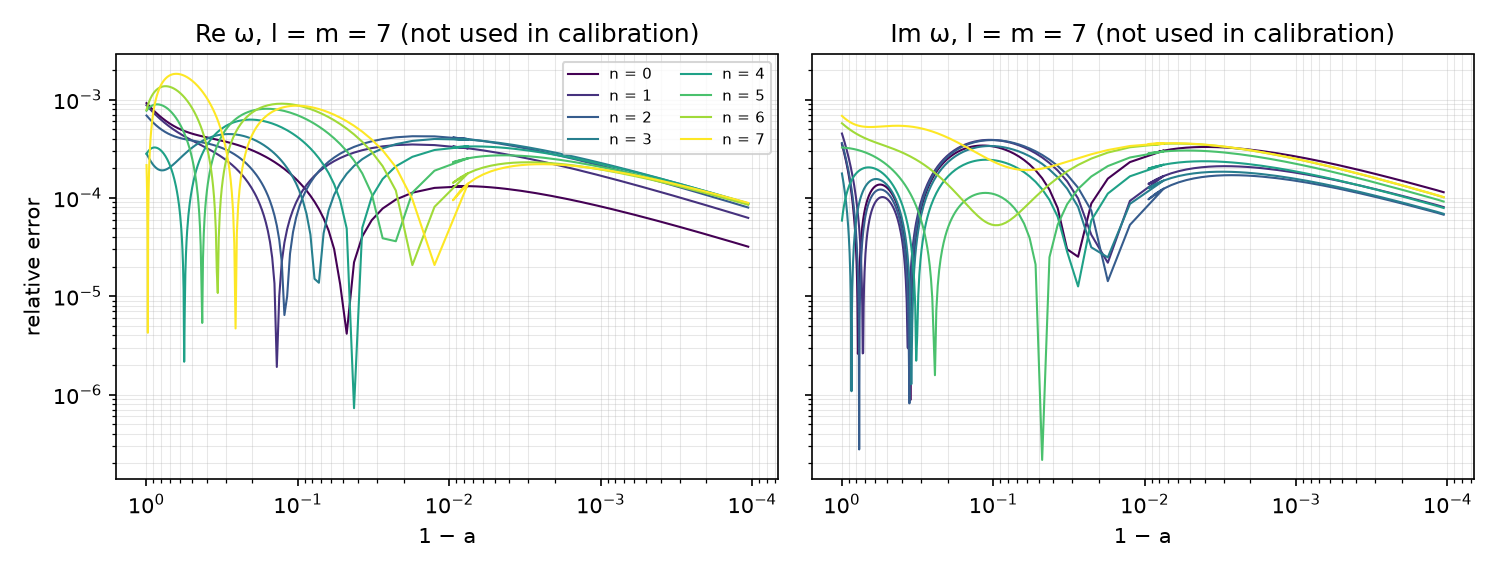
\includegraphics[width=\columnwidth]{fig_errors_l7.png}
\caption{Relative error of version B against $1-a$ for $l=m=7$, a mode never used in the calibration, for overtones
$n=0$--$7$ on the validation grid. Left: $\omega_R$; right: $\omega_I$.}
\label{fig:l7}
\end{figure}

\textit{Comparison with the competitors.} The single formula is calibrated once across modes. It still beats BCW and
two-term London, both calibrated per mode, on every mode, including modes it never saw. For $l\ge5$, version~B is
also more accurate on $\omega_I$ than the five-term London fit, which uses 80 numbers per mode. On $\omega_R$ the
five-term fit remains 5--15 times more accurate.

\textit{Overtones and spin.} The worst errors occur at the highest overtones. Figure~\ref{fig:l7} shows that the error
for the unseen $l=7$ mode stays below $0.2\%$ at all spins and overtones. For $l=2$, version~C beats even the
five-term London fit, with fewer numbers; its error is below $0.2\%$ for $n\le2$ and is dominated by $n=4$.

\textit{Extrapolation in $l$.} Away from the calibration range, the accuracy of version B degrades smoothly, from
$0.37\%/0.16\%$ at $l=8$ to $1.48\%/0.66\%$ at $l=12$.

\textit{A negative result.} During exploration we tried giving version B the richer second-order correction of
Eq.~(\ref{eq:corrC}). It improved the fit on calibration modes ($0.12\%/0.13\%$) but degraded the prediction of an
unseen mode, from $0.13\%/0.16\%$ to $0.81\%/0.82\%$. We therefore keep first order for the cross-mode formula.

%---------------------------------------------------------------------------------------------------------------
\section{Limitations}\label{sec:limits}

\begin{itemize}
\item Only prograde $l=m$ modes are covered. For $m<l$, damped and zero-damping branches coexist near extremality
and overtones can cross~\cite{Yang:2012pj,Cook:2014cta}. Our attempts to extend the tracking to $(2,1)$, $(3,2)$ and
$(4,3)$ did not yield reliable sequences.
\item The errors are maximum relative errors on a finite grid up to $a=0.9999$. We make no claim beyond that spin,
where the expansions of Ref.~\cite{Cook:2014cta} are the appropriate tool.
\item Per-mode, many-parameter fits remain more accurate on $\omega_R$. Interpolation of tabulated
data~\cite{Stein:2019mop} is more accurate still, but it is not a closed form.
\end{itemize}

%---------------------------------------------------------------------------------------------------------------
\section{Conclusions}

Two physically motivated bases, the light-ring Lyapunov exponent for the damping and the extremal value $m/2$ for the
frequency, combined with one rational correction in $\sqrt{1-a}$, yield a compact formula for Kerr $l=m$ overtones.
It holds over the whole spin range up to $a=0.9999$ and transfers to $l$ values outside its calibration set. The
fitting coefficients and a reference implementation are given below.

\begin{acknowledgments}
Exact frequencies were computed with the \texttt{qnm} package~\cite{Stein:2019mop}. Large parts of the code and text
were drafted with the assistance of an AI system (Claude, Anthropic). All results were produced by the preregistered
scripts described above and checked by the author.
\end{acknowledgments}

\appendix
\section{Coefficients}\label{app:coef}
\begin{table*}[t]\centering\footnotesize
\caption{Coefficients of version A. Each coefficient $X$ of Eq.~(\ref{eq:coef}) is $X=\sum_{j=0}^{2} n^j(\alpha_j+\beta_j/L+\gamma_j/L^2)$, $L=l+\tfrac12$.}
\label{tab:coefA}
\begin{tabular}{cc rrr}\hline\hline
coefficient & $j$ & $\alpha_j$ & $\beta_j$ & $\gamma_j$ \\ \hline
$A$ & 0 & $\phantom{-}0.0765154722$ & $-1.5516059526$ & $\phantom{-}2.2348079615$ \\
$A$ & 1 & $\phantom{-}0.0272471922$ & $-0.2188339970$ & $\phantom{-}0.5459416775$ \\
$A$ & 2 & $-0.0003739376$ & $-0.0058401195$ & $-0.0117864489$ \\
$B$ & 0 & $-0.0466468501$ & $\phantom{-}1.0528659907$ & $-1.5949762742$ \\
$B$ & 1 & $-0.0173349079$ & $\phantom{-}0.1904554267$ & $-0.3221004260$ \\
$B$ & 2 & $-0.0104359118$ & $\phantom{-}0.1259328761$ & $-0.2261158947$ \\
$C$ & 0 & $\phantom{-}5.2362345759$ & $-22.4469795148$ & $\phantom{-}22.6796309587$ \\
$C$ & 1 & $-0.5841838756$ & $\phantom{-}2.3817606585$ & $-3.8356208165$ \\
$C$ & 2 & $\phantom{-}0.0082582974$ & $\phantom{-}0.1921446130$ & $-0.2711354306$ \\
\hline
$D$ & 0 & $-1.1007091997$ & $-0.4635650254$ & $-1.3767592276$ \\
$D$ & 1 & $-0.0079989019$ & $-0.1305087380$ & $\phantom{-}1.1807109300$ \\
$D$ & 2 & $-0.0108536929$ & $\phantom{-}0.1462319274$ & $-0.5198674256$ \\
$E$ & 0 & $\phantom{-}0.2363956433$ & $-1.8346777585$ & $\phantom{-}3.1990739518$ \\
$E$ & 1 & $-0.1243398498$ & $\phantom{-}0.8344003079$ & $-0.6727072175$ \\
$E$ & 2 & $\phantom{-}0.0568530024$ & $-0.4533426932$ & $\phantom{-}0.6027971977$ \\
$F$ & 0 & $\phantom{-}0.3229097090$ & $\phantom{-}5.1547444199$ & $-6.2666445734$ \\
$F$ & 1 & $\phantom{-}0.2199421885$ & $-1.1356081561$ & $-1.2989614607$ \\
$F$ & 2 & $-0.0658233493$ & $\phantom{-}0.4089394719$ & $-0.0685837171$ \\
\hline
\hline\end{tabular}\end{table*}
\begin{table*}[t]\centering\footnotesize
\caption{Coefficients of version B. Each coefficient $X$ of Eq.~(\ref{eq:coef}) is $X=\sum_{j=0}^{3} n^j(\alpha_j+\beta_j/L+\gamma_j/L^2)$, $L=l+\tfrac12$.}
\label{tab:coefB}
\begin{tabular}{cc rrr}\hline\hline
coefficient & $j$ & $\alpha_j$ & $\beta_j$ & $\gamma_j$ \\ \hline
$A$ & 0 & $\phantom{-}0.0680773554$ & $-1.5090255390$ & $\phantom{-}2.2152780020$ \\
$A$ & 1 & $\phantom{-}0.0011881221$ & $\phantom{-}0.0347616704$ & $-0.0521028120$ \\
$A$ & 2 & $\phantom{-}0.0009984683$ & $-0.0194683604$ & $\phantom{-}0.0118291259$ \\
$A$ & 3 & $-0.0002596576$ & $\phantom{-}0.0035393176$ & $-0.0061409599$ \\
$B$ & 0 & $-0.0440253862$ & $\phantom{-}1.0411537116$ & $-1.5902996397$ \\
$B$ & 1 & $-0.0048704210$ & $\phantom{-}0.0704963287$ & $-0.0813431640$ \\
$B$ & 2 & $-0.0050543822$ & $\phantom{-}0.0835293547$ & $-0.1049293141$ \\
$B$ & 3 & $\phantom{-}0.0005616853$ & $-0.0085870525$ & $\phantom{-}0.0155068417$ \\
$C$ & 0 & $\phantom{-}6.1291458810$ & $-29.3628377321$ & $\phantom{-}35.4529776028$ \\
$C$ & 1 & $-0.8476399030$ & $\phantom{-}4.2402837113$ & $-6.4283578092$ \\
$C$ & 2 & $\phantom{-}0.0512535262$ & $-0.2600405485$ & $\phantom{-}0.7256841443$ \\
$C$ & 3 & $-0.0029801198$ & $\phantom{-}0.0176456278$ & $-0.0440477042$ \\
\hline
$D$ & 0 & $-1.2321297032$ & $\phantom{-}0.6810572043$ & $-3.6313321435$ \\
$D$ & 1 & $\phantom{-}0.1218795065$ & $-1.3770170681$ & $\phantom{-}3.6907288245$ \\
$D$ & 2 & $-0.0451282048$ & $\phantom{-}0.5098072566$ & $-1.3319396049$ \\
$D$ & 3 & $\phantom{-}0.0035849339$ & $-0.0409688119$ & $\phantom{-}0.1089269672$ \\
$E$ & 0 & $\phantom{-}0.0427796939$ & $-0.1755448719$ & $\phantom{-}0.0654161720$ \\
$E$ & 1 & $\phantom{-}0.1551146247$ & $-1.7442175894$ & $\phantom{-}4.4503119784$ \\
$E$ & 2 & $-0.0405044597$ & $\phantom{-}0.4858518647$ & $-1.5022013045$ \\
$E$ & 3 & $\phantom{-}0.0022044457$ & $-0.0341005912$ & $\phantom{-}0.1338287533$ \\
$F$ & 0 & $\phantom{-}0.9083355899$ & $\phantom{-}0.0878678986$ & $\phantom{-}3.5709337389$ \\
$F$ & 1 & $-0.4733391337$ & $\phantom{-}5.3346493974$ & $-14.0999861011$ \\
$F$ & 2 & $\phantom{-}0.1487222212$ & $-1.6974797904$ & $\phantom{-}4.4779672671$ \\
$F$ & 3 & $-0.0097700329$ & $\phantom{-}0.1192739776$ & $-0.3487927545$ \\
\hline
\hline\end{tabular}\end{table*}
\begin{table*}[t]\centering\footnotesize
\caption{Coefficients of version C ($l=m=2$). Each coefficient is $X=\sum_{j=0}^{3}x_j n^j$; the correction is Eq.~(\ref{eq:corrC}).}
\label{tab:coefC}
\begin{tabular}{cc rrrr}\hline\hline
part & coefficient & $x_0$ & $x_1$ & $x_2$ & $x_3$ \\ \hline
$\omega_I$ & $A'$ & $-0.1462609672$ & $-0.0153246711$ & $\phantom{-}0.0072868387$ & $\phantom{-}0.0006707917$ \\
$\omega_I$ & $B'$ & $\phantom{-}0.0529838739$ & $\phantom{-}0.1599833539$ & $-0.0261327479$ & $-0.0044078146$ \\
$\omega_I$ & $C'$ & $\phantom{-}0.0020794786$ & $-0.0522335160$ & $-0.0141524918$ & $\phantom{-}0.0083278271$ \\
$\omega_I$ & $D'$ & $-0.6438751286$ & $-0.4603515275$ & $\phantom{-}0.0998686926$ & $-0.0169603977$ \\
$\omega_I$ & $E'$ & $\phantom{-}0.8482123216$ & $-0.4466865157$ & $\phantom{-}0.1549523931$ & $-0.0011528525$ \\
\hline
$\omega_R$ & $A''$ & $-1.4510681813$ & $\phantom{-}0.0107928166$ & $-0.0004234928$ & $\phantom{-}0.0022111089$ \\
$\omega_R$ & $B''$ & $\phantom{-}0.6134050188$ & $\phantom{-}0.8539589180$ & $-0.4115399960$ & $\phantom{-}0.0324819406$ \\
$\omega_R$ & $C''$ & $-0.0532904184$ & $-0.1123371701$ & $\phantom{-}0.1406763788$ & $-0.0473275375$ \\
$\omega_R$ & $D''$ & $\phantom{-}0.8026997212$ & $-0.6743146313$ & $\phantom{-}0.2945831225$ & $-0.0420147162$ \\
$\omega_R$ & $E''$ & $-0.3801482070$ & $-0.5919957293$ & $\phantom{-}0.2037546838$ & $\phantom{-}0.0339572334$ \\
\hline
\hline\end{tabular}\end{table*}


\begin{thebibliography}{99}
\bibitem{Berti:2009kk} E.~Berti, V.~Cardoso and A.~O.~Starinets, Class.\ Quant.\ Grav.\ \textbf{26}, 163001 (2009),
arXiv:0905.2975.
\bibitem{Giesler:2019uxc} M.~Giesler, M.~Isi, M.~A.~Scheel and S.~A.~Teukolsky, Phys.\ Rev.\ X \textbf{9}, 041060
(2019), arXiv:1903.08284.
\bibitem{Leaver:1985ax} E.~W.~Leaver, Proc.\ R.\ Soc.\ Lond.\ A \textbf{402}, 285 (1985).
\bibitem{Stein:2019mop} L.~C.~Stein, J.\ Open Source Softw.\ \textbf{4}, 1683 (2019), arXiv:1908.10377.
\bibitem{Berti:2005ys} E.~Berti, V.~Cardoso and C.~M.~Will, Phys.\ Rev.\ D \textbf{73}, 064030 (2006),
arXiv:gr-qc/0512160.
\bibitem{London:2018nxs} L.~London and E.~Fauchon-Jones, Class.\ Quant.\ Grav.\ \textbf{36}, 235015 (2019),
arXiv:1810.03550.
\bibitem{Hod:2008zz} S.~Hod, Phys.\ Rev.\ D \textbf{78}, 084035 (2008), arXiv:0811.3806.
\bibitem{Yang:2012pj} H.~Yang, F.~Zhang, A.~Zimmerman, D.~A.~Nichols, E.~Berti and Y.~Chen, Phys.\ Rev.\ D
\textbf{87}, 041502(R) (2013), arXiv:1212.3271.
\bibitem{Yang:2013uba} H.~Yang, A.~Zimmerman, A.~Zengino\u{g}lu, F.~Zhang, E.~Berti and Y.~Chen, Phys.\ Rev.\ D
\textbf{88}, 044047 (2013), arXiv:1307.8086.
\bibitem{Cook:2014cta} G.~B.~Cook and M.~Zalutskiy, Phys.\ Rev.\ D \textbf{90}, 124021 (2014), arXiv:1410.7698.
\bibitem{Hu:2026resum} J.~Hu, K.~Yagi and N.~Yunes, arXiv:2607.27043 (2026).
\bibitem{Cardoso:2008bp} V.~Cardoso, A.~S.~Miranda, E.~Berti, H.~Witek and V.~T.~Zanchin, Phys.\ Rev.\ D \textbf{79},
064016 (2009), arXiv:0812.1806.
\bibitem{Dolan:2010wr} S.~R.~Dolan, Phys.\ Rev.\ D \textbf{82}, 104003 (2010), arXiv:1007.5097.
\end{thebibliography}

\end{document}
